\section{Project Control}
\label{sec:control}

% Control Measures examined and critiqued
% ie change requests

Projects that have run late or overbudget often find that the steps to failure happened gradually.
The small extra costs or wasted days gradually added up to form a very large and significant
problem. Project control is about detecting these small deviations and then implementing corrective
actions that prevents a build up of small problems.\citepage{maylor2010}{page 291}

Any large software system is going to undergo change as it is developed. Requirements may change,
bugs have to be fixed as they appear, and original design decisions may turn out to be insufficient.
Therefore, a set of change management processes are required to ensure that the evolution of a
system is controlled and does not succumb to scope creep or other problems that would prevent
successful delivery of the software.\citepage{sommerville2011}{page 685}

For the Serenity project the change management process shown in Figure~\ref{fig:change_management}
was devised. This protocol was designed to allow stakeholders outside of the development team
to submit change requests for assessment. When a change request is received it would be evaluated
in terms of its cost and impact on the project requirements. If the change is accepted then a
notification is relayed to the whole development team and relevant stakeholders. All change requests
would be archived so that reasons for rejection or approval could be reviewed again in the future.

\begin{figure*}
	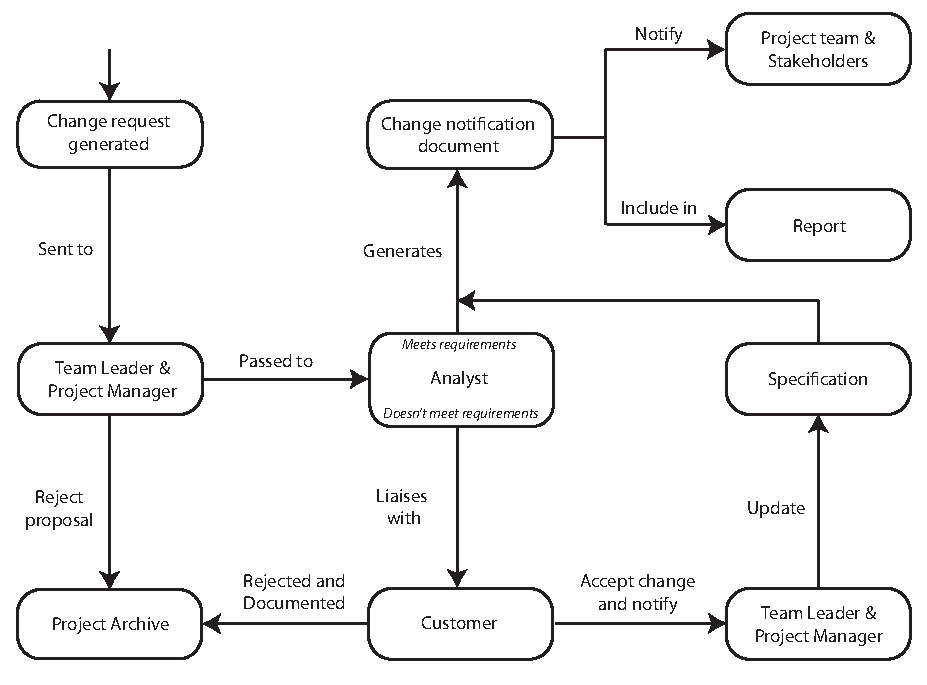
\includegraphics[height=33em]{res/change_management_diagram}
	\label{fig:change_management}
	\caption{Change management workflow}
\end{figure*}

In the end no change requests were submitted by any stakeholder not a part of the development team.
However, it is believed that this well documented and rigorous change management workflow would
have enabled the project to deal with any such change requests in an efficient manner.
Many minor changes, such as bug fixes, were discussed more informally within the development as
they had no effect on the schedule or requirements. This worked effectively whereas using the
formal change management procedure for such small changes would be overkill and lead to a lot
of time being wasted in communications overhead.

% Major changes? E.g. scaling back the goals to get a finished product.

A formalised change management workflow is necessary for a successful project, but it must only
be used where appropriate to ensure that it does not get in the way of smaller changes that
can be dealt with more informally.
